\newpage
\section{Нейронные сети}

Среди алгоритмов распознавания образов особое место занимают нейронные сети. Повышенный интерес к данной технологии в наши дни обусловлен успехами сетей в распознавании широкого класса паттернов, новыми численными методами для обучения многоуровневых нелинейных моделей и прогрессом в области производства недорогих и эффективных векторных процессоров для расчетов. При решении задач компьютерного зрения наибольшей популярностью пользуются сверточные нейронные сети (СНС). Модель СНС улучшает качество распознавания каскадного классификатора на ЛБШ за счет дополнительной фильтрации шумов.

В середине прошлого столетия ученые Торстен Визель и Дэвид Хьюбел исследовали зрительную кору головного мозга кошки и обнаружили, что существует два различных типа клеток. Так называемые простые клетки реагируют на прямые линии (полосы света, края стимулов) под определенным углом. Сложные клетки реагирую на движение линий (полос света, краев стимулов) в определенных направлениях. Спустя некоторое время, это открытие нашло применение в прикладной области информатики: Кунихика Фукусима воплотил идею простых и сложных клеток в неокогнитроне

\begin{figure}[h!]
\centering
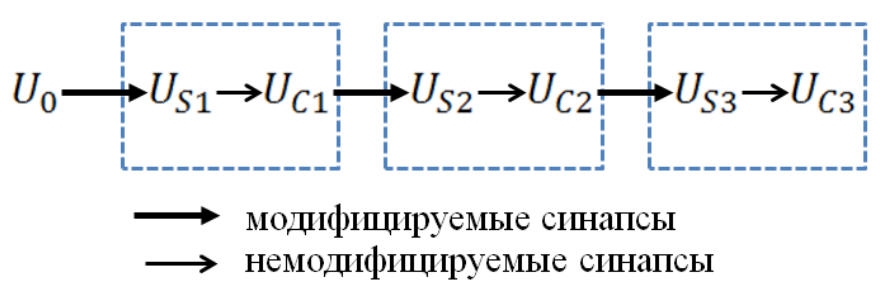
\includegraphics[scale=0.5]{res/pic012}
\caption{Упрощенная структура неокогнитрона}
\end{figure}

Неокогнитрон состоит из ретины (сетчатки) $U_0$ и последовательности групп нейронов, каждая из которых, в свою очередь, содержит два типа нейронных слоев (рис. 12). Простые нейроны (из слоев $U_S$) принимают сигналы от сложных нейронов предыдущего слоя и обнаруживают одинаковые признаки, но в разных местах сигнала. Сложные нейроны (из слоев $U_C$) объединяют отклики простых нейронов из своей группы и стремятся редуцировать зависимость реакции на признаки от их положения. Таким образом, неокогнитрон приобретает способность детектировать определенные комбинации признаков, независимо от их положения на ретине.

\begin{figure}[h!]
\centering
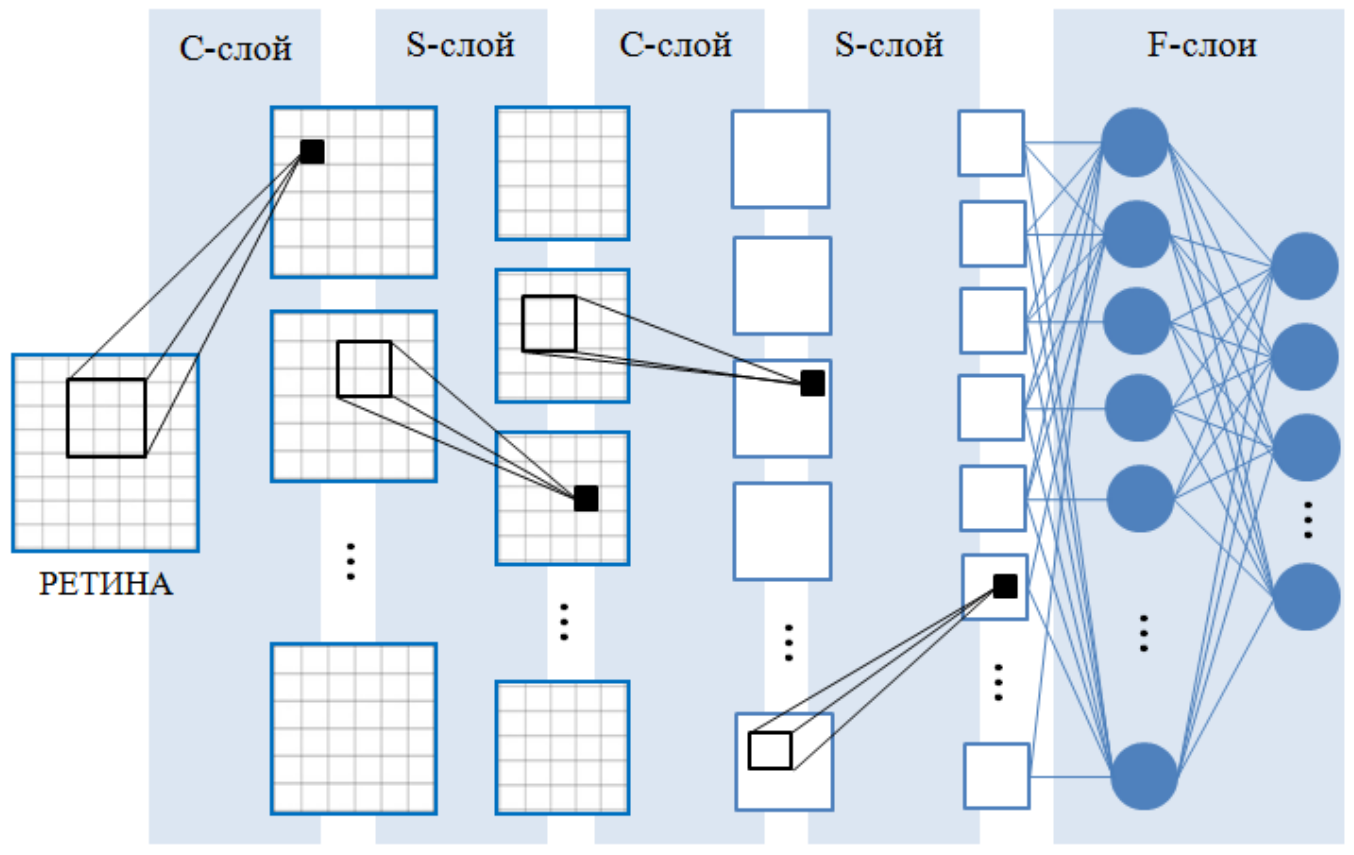
\includegraphics[scale=0.35]{res/pic013}
\caption{Архитектура сверточной нейронной сети}
\end{figure}

Отличие неокогнитрона от многослойного персептрона заключается в трех инновационных для нейронных сетей на тот момент архитектурных принципах:
\begin{itemize}
\item локальные рецептивные поля,
\item разделяемые веса,
\item пространственная субдискретизация.
\end{itemize}

Развивая идею неокогнитрона, Ян ЛеКун вместе с соавторами предложили структуру классической сверточной нейронной сети (СНС) и алгоритм для ее обучения с учителем, а также применение СНС для решения широкого круга задач распознавания образов. СНС, предложенные ЛеКуном (рис. 13), это иерархичные архитектурные многослойные идеи нейронные неокогнитрона, сети, в которых обеспечивающие сходятся некоторую три степень инвариантности представления данных.

Устройство СНС заключается в чередовании сверточных слоев (convolutional, C-слои), реализующих концепцию простых клеток зрительной коры с гибкими (обучаемыми) весами, и субдискретизирующих слоев (sub-sampling, S-слои), построенных по примеру сложных клеток кортекса с жесткими весами. Завершается подобная каскадная модель, как правило, полносвязными нейронными слоями (fully-connected, F-слои). Различные архитектуры СНС успешно используются во многих сложных приложениях, связанных с обработкой визуальных данных.